\begin{enumerate}
\item There is a group of six people: Ana, Josh, Hope, Patricia, Jeff, and Carlos.  Josh is friends with Patricia, Hope, and Ana; Jeff is friends with Patricia and Carlos; Patricia and Hope are friends.  None of the other pairs of people are friends.  Draw a graph to represent this group.
\begin{center}
\begin{tikzpicture}
  \GraphInit[vstyle=simple]
  \tikzset{VertexStyle/.append style={scale=0.3}}
  \SetGraphUnit{1.8}
  
  \Vertex{Ana}
  \EA(Ana){Josh}
  \SO(Ana){Hope}
  \SO(Josh){Patricia}
  \EA(Josh){Jeff}
  \SO(Jeff){Carlos}
  
  \extralabel[1mm]{Ana}{90}{Ana}
  \extralabel[1mm]{Josh}{90}{Josh}
  \extralabel[1mm]{Hope}{-90}{Hope}
  \extralabel[1mm]{Patricia}{-90}{Patricia}
  \extralabel[1mm]{Jeff}{90}{Jeff}
  \extralabel[1mm]{Carlos}{-90}{Carlos}
  
  %\tikzset{EdgeStyle/.style = {->-,>=latex[round]}}
  \Edge(Josh)(Patricia)
  \Edge(Josh)(Hope)
  \Edge(Josh)(Ana)
  \Edge(Jeff)(Patricia)
  \Edge(Jeff)(Carlos)
  \Edge(Patricia)(Hope)
\end{tikzpicture}
\end{center}

\item On campus, you travel between five buildings: Braddock Hall, Catoctin Hall, the library, the student center, and the arts building.  There are walkways connecting Braddock Hall to Catoctin Hall and the library; the library is also connected to the arts building and the student center; there are also walkways connecting the student center to Catoctin Hall and the arts building.  Draw a graph to represent this group of buildings.
\begin{center}
\begin{tikzpicture}
  \GraphInit[vstyle=simple]
  \tikzset{VertexStyle/.append style={scale=0.3}}
  \SetGraphUnit{1.8}
  
  \Vertex{Braddock}
  \EA(Braddock){Catoctin}
  \SO(Braddock){Library}
  \SO(Catoctin){SC}
  \EA(Catoctin){Arts}
  
  \extralabel[1mm]{Braddock}{90}{Braddock}
  \extralabel[1mm]{Catoctin}{90}{Catoctin}
  \extralabel[1mm]{Library}{-90}{Library}
  \extralabel[1mm]{SC}{-90}{Student Center}
  \extralabel[1mm]{Arts}{-90}{Arts}
  
  %\tikzset{EdgeStyle/.style = {->-,>=latex[round]}}
  \Edge(Braddock)(Catoctin)
  \Edge(Braddock)(Library)
  \Edge(Library)(Arts)
  \Edge(Library)(SC)
  \Edge(SC)(Catoctin)
  \Edge(SC)(Arts)
\end{tikzpicture}
\end{center}

\item The map below shows eight states and the District of Columbia highlighted in blue.  Draw a graph to represent this map, where each node represents a state or district, and an edge represents a shared border between two regions.
\begin{center}
\begin{tabular}{c c}
\includegraphics[height=1.5in]{selected_states_around_md_cropped}
&
\begin{tikzpicture}
  \GraphInit[vstyle=simple]
  \tikzset{VertexStyle/.append style={scale=0.3}}
  \SetGraphUnit{1.8}
  
  \grEmptyCycle[RA=2,prefix=a]{8}
  \grEmptyCycle[RA=0,prefix=b]{1}
  
  \extralabel[1mm]{a0}{0}{MD}
  \extralabel[1mm]{a1}{45}{DE}
  \extralabel[1mm]{a2}{90}{NJ}
  \extralabel[1mm]{a3}{135}{PA}
  \extralabel[1mm]{a4}{180}{OH}
  \extralabel[1mm]{a5}{225}{KY}
  \extralabel[1mm]{a6}{-90}{VA}
  \extralabel[1mm]{a7}{-45}{DC}
  \extralabel[1mm]{b0}{-45}{WV}
  
  %\tikzset{EdgeStyle/.style = {->-,>=latex[round]}}
  \Edge(a0)(a1)
  \Edge(a0)(a3)
  \Edge(a0)(a6)
  \Edge(a0)(a7)
  \Edge(a0)(b0)
  \Edge(a1)(a2)
  \Edge(a1)(a3)
  \Edge(a2)(a3)
  \Edge(a3)(a4)
  \Edge(a3)(b0)
  \Edge(a4)(a5)
  \Edge(a4)(b0)
  \Edge(a5)(a6)
  \Edge(a5)(b0)
  \Edge(a6)(a7)
  \Edge(a6)(b0)
\end{tikzpicture}
\end{tabular}
\end{center}
\pagebreak

\item The map below shows eight countries in Asia highlighted in blue.  Draw a graph to represent this map, where each node represents a country, and an edge represents a shared border between two countries.
\begin{center}
\begin{tabular}{c c}
\includegraphics[height=2in]{middle_east_countries_cropped}
&
\begin{tikzpicture}
  \GraphInit[vstyle=simple]
  \tikzset{VertexStyle/.append style={scale=0.3}}
  \SetGraphUnit{1.8}
  
  \grEmptyCycle[RA=2,prefix=a]{7}
  \grEmptyCycle[RA=0,prefix=b]{1}
  
  \extralabel[1mm]{a0}{0}{Taj.}
  \extralabel[1mm]{a1}{45}{Kyr.}
  \extralabel[1mm]{a2}{90}{Kaz.}
  \extralabel[1mm]{a3}{135}{Uzb.}
  \extralabel[1mm]{a4}{180}{Tur.}
  \extralabel[1mm]{a5}{225}{Iran}
  \extralabel[1mm]{a6}{-90}{Pak.}
  \extralabel[1mm]{b0}{-45}{Afg.}
  
  %\tikzset{EdgeStyle/.style = {->-,>=latex[round]}}
  \Edge(a0)(a1)
  \Edge(a0)(a3)
  \Edge(a0)(b0)
  \Edge(a1)(a2)
  \Edge(a1)(a3)
  \Edge(a2)(a3)
  \Edge(a2)(a4)
  \Edge(a3)(a4)
  \Edge(a3)(b0)
  \Edge(a4)(a5)
  \Edge(a4)(b0)
  \Edge(a5)(a6)
  \Edge(a5)(b0)
  \Edge(a6)(b0)
\end{tikzpicture}
\end{tabular}
\end{center}

\item The graph below represents a tournament; each edge marks a game between two teams.
\begin{center}
\begin{tikzpicture}
  \GraphInit[vstyle=simple]
  \tikzset{VertexStyle/.append style={scale=0.3}}
  \SetGraphUnit{1}
  
  \grEmptyCycle[RA=1.5,rotation=18,prefix=a]{5}
  
  \extralabel[1mm]{a0}{0}{Warriors}
  \extralabel[1mm]{a1}{90}{Hawks}
  \extralabel[1mm]{a2}{180}{Hornets}
  \extralabel[1mm]{a3}{-90}{Lions}
  \extralabel[1mm]{a4}{-90}{Bears}
  
  \Edge(a1)(a0)
  \Edge(a1)(a3)
  \Edge(a2)(a4)
  \Edge(a2)(a0)
  \Edge(a4)(a0)
  \Edge(a2)(a3)
  \Edge(a0)(a3)
\end{tikzpicture}
\end{center}
\begin{enumerate}[(a)]
\item Did the Hornets and the Hawks play each other? \answersub{No}
\item How many games do the Warriors play? \answersub{4}
\item Which teams do the Bears play? \answersub{Hornets and Warriors}
\item Which team(s) played the most games? \answersub{Warriors}
\item Which team(s) played the fewest games? \answersub{Hawks and Bears (each played 2)}
\end{enumerate}

\item The graph below is an \emph{influence graph}, where each edge represents the influence that one person has on another; the arrow goes from the influencer to the one they influence.
\begin{center}
\begin{tikzpicture}
  \GraphInit[vstyle=simple]
  \tikzset{VertexStyle/.append style={scale=0.3}}
  \SetGraphUnit{1.8}
  
  \Vertex{Joelle}
  \EA(Joelle){Jonathan}
  \SO(Joelle){Anastasia}
  \SO(Jonathan){Laila}
  \EA(Laila){Zachary}
  
  \extralabel[1mm]{Joelle}{90}{Joelle}
  \extralabel[1mm]{Jonathan}{90}{Jonathan}
  \extralabel[1mm]{Anastasia}{-90}{Anastasia}
  \extralabel[1mm]{Laila}{-90}{Laila}
  \extralabel[1mm]{Zachary}{0}{Zachary}
  
  \tikzset{EdgeStyle/.style = {->-,>=latex[round]}}
  \Edge(Zachary)(Jonathan)
  \Edge(Zachary)(Laila)
  \Edge(Zachary)(Joelle)
  \Edge(Anastasia)(Jonathan)
  \Edge(Joelle)(Laila)
  \Edge(Laila)(Jonathan)
  \Edge(Anastasia)(Joelle)
\end{tikzpicture}
\end{center}
\begin{enumerate}[(a)]
\item Who does Laila influence? \answersub{Jonathan}
\item Does Jonathan influence Anastasia? \answersub{No}
\item How many people does Joelle influence? \answersub{1}
\item Who is the most influential (influences the most people)? \answersub{Zachary (3)}
\item Who is the most influenced (influenced by the most people)? \answersub{Jonathan (3)}
\end{enumerate}
\end{enumerate}

\emph{For problems 7--10, describe a graph that could be used to model the given application.  Specifically, answer the following questions:
\begin{enumerate}[(a)]
\item Are loops allowed in this graph?
\item Are multiple edges allowed between the same pair of nodes?
\item Is this a simple graph or multigraph?
\item Is this graph directed or undirected?
\item Is this a complete graph (generally)?
\end{enumerate}}

\begin{enumerate}
\setcounter{enumi}{6}

\item Flights between major cities, if each node represents a city and each edge describes a flight from one city to another (or from a city to itself, if there is a sightseeing or training flight).
\begin{enumerate}[(a)]
\item Are loops allowed in this graph? \answersub{Yes}
\item Are multiple edges allowed between the same pair of nodes? \answersub{Yes}
\item Is this a simple graph or multigraph? \answersub{Multigraph}
\item Is this graph directed or undirected? \answersub{Directed}
\item Is this a complete graph (generally)? \answersub{No}
\end{enumerate}

\item A party, where each node represents a person, and each edge represents whether one person knows the name of another.
\begin{enumerate}[(a)]
\item Are loops allowed in this graph? \answersub{Yes}
\item Are multiple edges allowed between the same pair of nodes? \answersub{Yes}
\item Is this a simple graph or multigraph? \answersub{Multigraph}
\item Is this graph directed or undirected? \answersub{Directed}
\item Is this a complete graph (generally)? \answersub{No}
\end{enumerate}

\item The floorplan of a house, where each node represents a room or space (like a hallway), and each edge represents a doorway.
\begin{enumerate}[(a)]
\item Are loops allowed in this graph? \answersub{No}
\item Are multiple edges allowed between the same pair of nodes? \answersub{Yes}
\item Is this a simple graph or multigraph? \answersub{Multigraph}
\item Is this graph directed or undirected? \answersub{Undirected}
\item Is this a complete graph (generally)? \answersub{No}
\end{enumerate}

\item Courses offered at a college, where each node represents a course, and each edge represents a prerequisite requirement.
\begin{enumerate}[(a)]
\item Are loops allowed in this graph? \answersub{No}
\item Are multiple edges allowed between the same pair of nodes? \answersub{No}
\item Is this a simple graph or multigraph? \answersub{Simple}
\item Is this graph directed or undirected? \answersub{Directed}
\item Is this a complete graph (generally)? \answersub{No}
\end{enumerate}
\end{enumerate}

\emph{For problems 11--14, answer the following questions for the given graph:
\begin{enumerate}[(a)]
\item Is it a simple graph or multigraph?
\item Is it directed or undirected?
\end{enumerate}}

\begin{enumerate}
\setcounter{enumi}{10}

\item \text{} \answer{(a) Multigraph (b) Undirected} 
\begin{center}
\begin{tikzpicture}
  \GraphInit[vstyle=simple]
  \tikzset{VertexStyle/.append style={scale=0.3}}
  \SetGraphUnit{2.2}
  
  \Vertex{a}
  \EA(a){b}
  \SO(a){c}
  \SO(b){d}
  
  \extralabel[1mm]{a}{90}{$a$}
  \extralabel[1mm]{b}{90}{$b$}
  \extralabel[1mm]{c}{-90}{$c$}
  \extralabel[1mm]{d}{-90}{$d$}
  
  %\tikzset{EdgeStyle/.style = {->-,>=latex[round]}}
  %\SetUpEdge[style={bend right=30}]
  %\Loop[dist=1.5cm,dir=NO,style={-}](NYC)
  \Edge(a)(b)
  \Edge(b)(d)
  \Edge(b)(c)
  \SetUpEdge[style={bend right=30}]
  \Edge(a)(d)
  \Edge(d)(a)
\end{tikzpicture}
\end{center}

\item \text{} \answer{(a) Multigraph (b) Directed} 
\begin{center}
\begin{tikzpicture}
  \GraphInit[vstyle=simple]
  \tikzset{VertexStyle/.append style={scale=0.3}}
  \SetGraphUnit{2.2}
  
  \Vertex{a}
  \EA(a){b}
  \SO(a){c}
  \SO(b){d}
  
  \extralabel[1mm]{a}{90}{$a$}
  \extralabel[1mm]{b}{90}{$b$}
  \extralabel[1mm]{c}{-90}{$c$}
  \extralabel[1mm]{d}{-90}{$d$}
  
  \tikzset{EdgeStyle/.style = {->-,>=latex[round]}}
  %\SetUpEdge[style={bend right=30}]
  %\Loop[dist=1.5cm,dir=NO,style={-}](NYC)
  \Edge(a)(c)
  \Edge(b)(c)
  \Edge(d)(b)
  \tikzset{EdgeStyle/.style = {->-,>=latex[round],bend right=30}}
  \Edge(a)(b)
  \Edge(b)(a)
\end{tikzpicture}
\end{center}

\item \text{} \answer{(a) Multigraph (b) Undirected} 
\begin{center}
\begin{tikzpicture}
  \GraphInit[vstyle=simple]
  \tikzset{VertexStyle/.append style={scale=0.3}}
  \SetGraphUnit{0.75}
  
  \Vertex{a}
  \EA(a){b}
  \SOEA(b){c}
  \SOWE(c){d}
  \WE(d){e}
  \NOWE(e){f}
  
  \extralabel[1mm]{a}{90}{$a$}
  \extralabel[1mm]{b}{0}{$b$}
  \extralabel[1mm]{c}{0}{$c$}
  \extralabel[1mm]{d}{-90}{$d$}
  \extralabel[1mm]{e}{-90}{$e$}
  \extralabel[1mm]{f}{180}{$f$}
  
  %\tikzset{EdgeStyle/.style = {->-,>=latex[round]}}
  %\SetUpEdge[style={bend right=30}]
  \Loop[dist=1.2cm,dir=NO,style={-}](b)
  \Loop[dist=1.2cm,dir=WE,style={-}](e)
  \Edge(a)(b)
  \Edge(a)(b)
  \Edge(b)(c)
  \SetUpEdge[style={bend right=15}]
  \Edge(a)(d)
  \Edge(d)(a)
  \Edge(a)(e)
  \Edge(e)(f)
  \Edge(a)(d)
  \Edge(c)(f)
\end{tikzpicture}
\end{center}

\item \text{} \answer{(a) Simple graph (b) Directed} 
\begin{center}
\begin{tikzpicture}
  \GraphInit[vstyle=simple]
  \tikzset{VertexStyle/.append style={scale=0.3}}
  \SetGraphUnit{1.8}
  
  \Vertex{a}
  \EA(a){b}
  \SO(a){c}
  \SO(b){d}
  \EA(b){e}
  
  \extralabel[1mm]{a}{90}{$a$}
  \extralabel[1mm]{b}{90}{$b$}
  \extralabel[1mm]{c}{-90}{$c$}
  \extralabel[1mm]{d}{-90}{$d$}
  \extralabel[1mm]{e}{0}{$e$}
  
  \tikzset{EdgeStyle/.style = {->-,>=latex[round]}}
  \Edge(a)(b)
  \Edge(c)(a)
  \Edge(a)(d)
  \Edge(b)(e)
  \Edge(e)(d)
  \Edge(d)(b)
\end{tikzpicture}
\end{center}
\end{enumerate}

\emph{For problems 15--17, determine the degree of each node.  For the directed graphs, determine both the in-degree and the out-degree of each node.}

\begin{enumerate}
\setcounter{enumi}{14}

\item \text{} \begin{center}
\begin{tikzpicture}
  \GraphInit[vstyle=simple]
  \tikzset{VertexStyle/.append style={scale=0.3}}
  \SetGraphUnit{2}
  
  \Vertex{a}
  \EA(a){b}
  \SO(a){c}
  \SO(b){d}
  \EA(b){e}
  
  \extralabel[1mm]{a}{90}{$a$}
  \extralabel[1mm]{b}{90}{$b$}
  \extralabel[1mm]{c}{-90}{$c$}
  \extralabel[1mm]{d}{-90}{$d$}
  \extralabel[1mm]{e}{0}{$e$}
  
  \tikzset{EdgeStyle/.style = {->-,>=latex[round]}}
  \Loop[dist=1.2cm,dir=NO,style={->-}](b)
  \Edge(b)(c)
  \Edge(d)(e)
  \Edge(d)(b)
  \tikzset{EdgeStyle/.style = {->-,>=latex[round],bend right=15}}
  \Edge(a)(c)
  \Edge(c)(a)
  \Edge(b)(e)
  \Edge(e)(b)
\end{tikzpicture}
\end{center}
\begin{center}
\begin{tabular}{c c c}
\textbf{Node} & \textbf{In-Degree} & \textbf{Out-Degree}\\
\hline
$a$ & 1 & 1\\
$b$ & 3 & 3\\
$c$ & 2 & 1\\
$d$ & 0 & 2\\
$e$ & 2 & 1
\end{tabular}
\end{center}

\item \text{} \begin{center}
\begin{tikzpicture}
  \GraphInit[vstyle=simple]
  \tikzset{VertexStyle/.append style={scale=0.3}}
  
  \grEmptyCycle[RA=1.7,prefix=a]{6}
  
  \extralabel[1mm]{a0}{0}{$a$}
  \extralabel[1mm]{a1}{90}{$b$}
  \extralabel[1mm]{a2}{90}{$c$}
  \extralabel[1mm]{a3}{180}{$d$}
  \extralabel[1mm]{a4}{-90}{$e$}
  \extralabel[1mm]{a5}{-90}{$f$}
  
  %\tikzset{EdgeStyle/.style = {->-,>=latex[round]}}
  %\SetUpEdge[style={bend right=30}]
  %\Loop[dist=1.5cm,dir=NO,style={-}](NYC)
  \Edge(a0)(a1)
  \Edge(a0)(a3)
  \Edge(a1)(a4)
  \Edge(a2)(a4)
  \Edge(a3)(a5)
  \SetUpEdge[style={bend right=20}]
  \Edge(a1)(a5)
  \Edge(a5)(a1)
\end{tikzpicture}
\end{center}
\begin{center}
\begin{tabular}{c c}
\textbf{Node} & \textbf{Degree}\\
\hline
$a$ & 2\\
$b$ & 4\\
$c$ & 1\\
$d$ & 2\\
$e$ & 2\\
$f$ & 3
\end{tabular}
\end{center}
\pagebreak

\item \text{} \begin{center}
\begin{tikzpicture}
  \GraphInit[vstyle=simple]
  \tikzset{VertexStyle/.append style={scale=0.3}}
  \grComplete[RA=1.7,prefix=a]{7}
  
  \extralabel[1mm]{a0}{0}{$a$}
  \extralabel[1mm]{a1}{45}{$b$}
  \extralabel[1mm]{a2}{90}{$c$}
  \extralabel[1mm]{a3}{135}{$d$}
  \extralabel[1mm]{a4}{180}{$e$}
  \extralabel[1mm]{a5}{-90}{$f$}
  \extralabel[1mm]{a6}{-45}{$g$}
\end{tikzpicture}
\end{center}
\begin{center}
\begin{tabular}{c c}
\textbf{Node} & \textbf{Degree}\\
\hline
$a$ & 6\\
$b$ & 6\\
$c$ & 6\\
$d$ & 6\\
$e$ & 6\\
$f$ & 6\\
$g$ & 6
\end{tabular}
\end{center}
\end{enumerate}